\section{The model}
\label{sec:the-model}
In this section we will go through the model presented in \cite{self-org} in 
detail. As mentioned in the introduction, social force models are agent-based, 
that is they describe the system by looking at the behaviour of each agent or, 
in our case, pedestrian in the system.


In this model the behaviour each pedestrian is defined by a series of social 
forces. We will describe three main forces, that each represent a tendency of 
the pedestrians. These forces are \emph{the desired movement force},  
\emph{the interaction force} between pedestrians and \emph{the repulsive 
force}  from the walls. The model also contains an attractive force, allowing 
e.g. a group of pedestrians to stick together when moving around, and a 
fluctuation term, adding a stochastic quality to the model. Both these forces, 
however, are only mentioned in the article, and are not really used. We have 
written the authors of the article asking about this, and they have replied 
that these parts of the model have not been used in practice, but that they 
might be useful to include at a later point in time.  Because of this, we will 
exclude these parts from the explanation of the model.

In the following, we will go through the three main forces, explaining how 
they are calculated. Since the notation used in the article is ambiguous and 
confusing, we introduce our own notation in an attempt to make it clearer. We 
will not refer to the original notation, but only use our own.

In the model, a pedestrian is represented by a circle with a centre, a radius 
and a current velocity. Walls are represented as line segments. The desired 
direction is represented by assigning to each pedestrian a target to move 
towards. Various other parameters are assigned to each pedestrian; these will 
be explained when relevant throughout the description. The notation for 
pedestrians and the main forces acting on a pedestrian are illustrated in  
figure~\ref{pedestrian-notation}.  

\begin{figure}[ht]
    \centering
    \subfloat[Notation of pedestrian properties.]{
        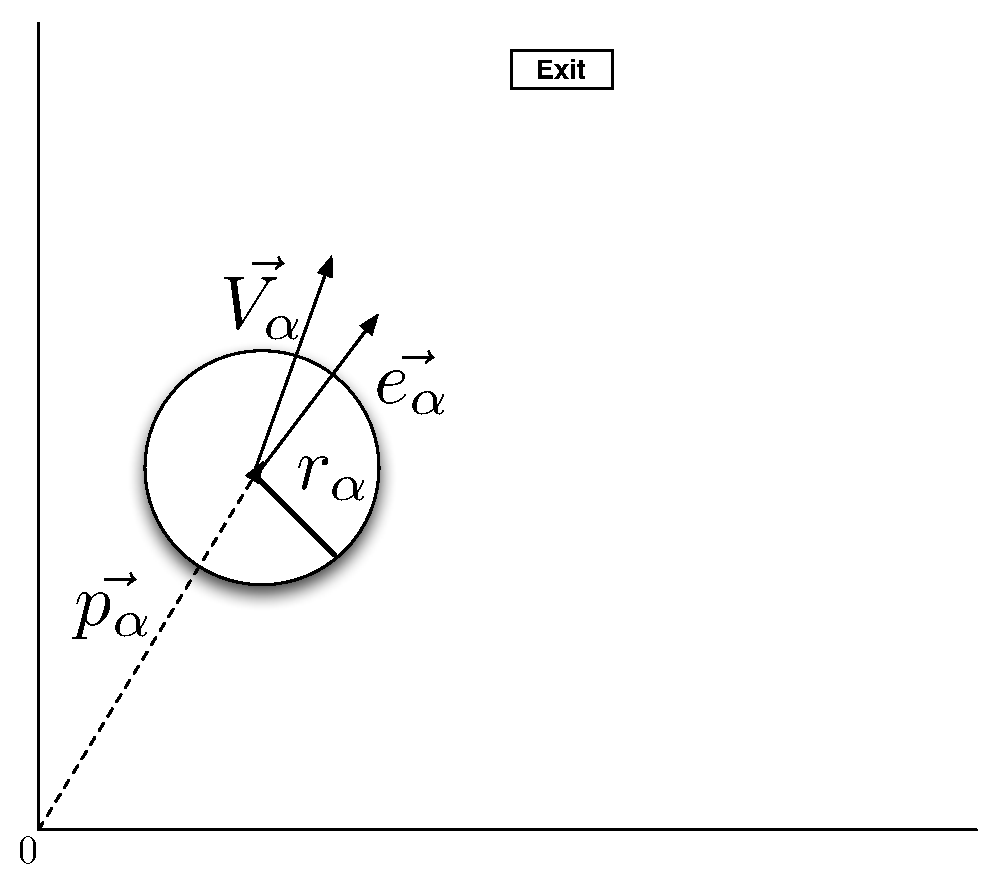
\includegraphics[width=0.45\textwidth]{Figures/NotationOfPedestrian.pdf}
        \label{subfig:notation}
    }
    \subfloat[Main forces acting on a pedestrian.]{
        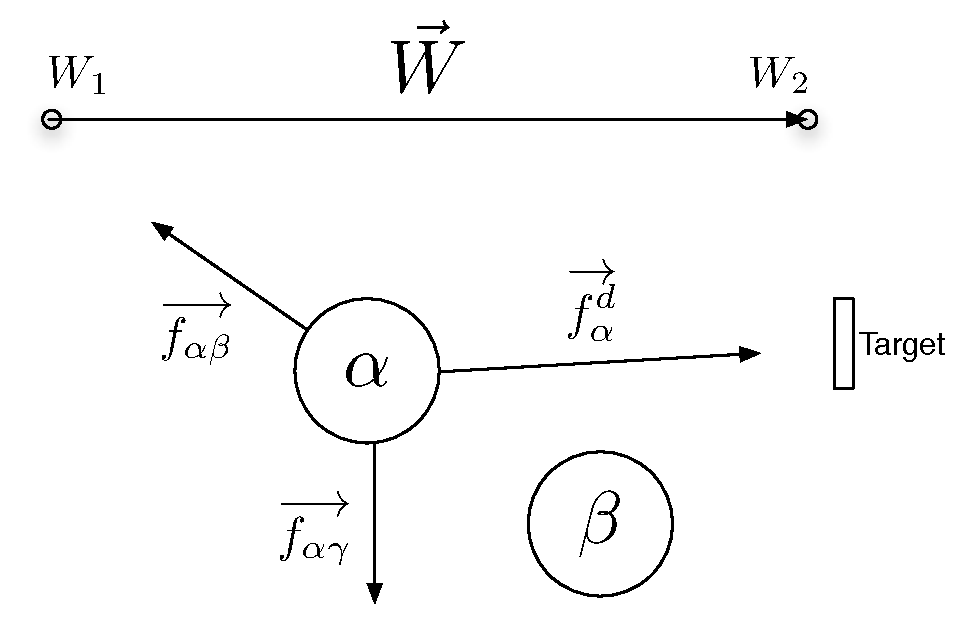
\includegraphics[width=0.45\textwidth]{Figures/ForceModel.pdf}
        \label{subfig:forces}
    }
    \caption[Notation for pedestrians]{Notation for a pedestrian.  
    \subref{subfig:notation} The notation for pedestrian properties. Position 
    vector ($ \overrightarrow{p_{\alpha}} $), velocity vector ($ 
    \overrightarrow{V_{\alpha}} $), vector pointing towards 
    the target ($\overrightarrow{e_{\alpha}}$)  and radius ($ R_{\alpha} $).
    %
    \subref{subfig:forces} Main forces acting on a pedestrian $\alpha$. 
    Interaction force from pedestrian $\beta$ 
    ($\overrightarrow{f_{\alpha\beta}}$), repulsive force from wall $\gamma$ 
    ($\overrightarrow{f_{\alpha \gamma}}$) and desired force towards target 
    ($\overrightarrow{f^{d}_{\alpha}}$).}

    \label{pedestrian-notation}
\end{figure}

The resulting force for pedestrian $\alpha$, $\overrightarrow{f_{\alpha}}$ is 
the sum of the three main forces:

\begin{equation}\label{model}
    \overrightarrow{f_{\alpha}} = \overrightarrow{f^{d}_{\alpha}} +
    \sum_{\beta \neq \alpha} \overrightarrow{f_{\alpha \beta}} +
    \sum_{\gamma} \overrightarrow{f_{\alpha \gamma}}
\end{equation}

Here $\overrightarrow{f_{\alpha}^{d}}$ is the desired force,  
$\overrightarrow{f_{\alpha \beta}}$ is the interaction force from pedestrian 
$\beta$ and $\overrightarrow{f_{\alpha \gamma}}$ is the repulsive force from 
wall $\gamma$. The main forces are summarised in table~\ref{tbl:main-forces} 
and will be described in detail in the following sections.

\begin{table}[h]
    \centering
    \begin{tabular}{l l}
        \toprule
        \multicolumn{2}{c}{\textsf{Main forces}}\\
        $\overrightarrow{f_{\alpha}^{d}}$ & Desired force\\
        $\overrightarrow{f_{\alpha \beta}}$ & Interaction force from pedestrian 
        $\beta$\\
        $\overrightarrow{f_{\alpha \gamma}}$ & Repulsive force from wall 
        $\gamma$\\
        \midrule
        \multicolumn{2}{c}{\textsf{Base notation}}\\
        $\overrightarrow{p_{\alpha}}$ & Position vector of pedestrian 
        $\alpha$\\
        $\overrightarrow{V_{\alpha}}$ & Velocity of pedestrian $\alpha$ \\ 
        \addlinespace[0.3em]
        $R_\alpha$ & Radius of pedestrian $\alpha$\\
        \bottomrule
    \end{tabular}
    \caption{Summary of main forces and base notation.}
    \label{tbl:main-forces}
\end{table}

\subsection{The desired force}
\label{sec:desired-force}
The \emph{desired force} represents the pedestrians' desire to move towards its 
target. The idea is that a pedestrian, if unhindered, will move towards its 
target at an initial desired speed that is given as a model parameter. The 
desired force is a velocity dependent force given by:

\begin{equation}\label{eqn:desired-force}
	\overrightarrow{f^{d}_{\alpha}} (t) =
    \frac{1}{\tau}
    \left( V_{\alpha}^{d}(t) \overrightarrow{e_{\alpha}} - 
    \overrightarrow{V_{\alpha}}(t) \right)
\end{equation}

Here $V_{\alpha}^{d}(t)$ is the desired speed at time $t$, 
$\overrightarrow{e_{\alpha}}$ is the unit vector pointing towards the 
pedestrian's target and  $\overrightarrow{V_{\alpha}}(t)$ is the actual 
velocity of the pedestrian at time $t$. It is not clear from the article what 
the initial velocity of the pedestrians is (i.e.  
$\overrightarrow{V_\alpha}(0)$), so we have assumed it to be zero.


$\tau$ is the \emph{relaxation time} and determines how fast a pedestrian 
returns to its desired velocity after having been walking slower because of 
obstacles etc. The relaxation time is a model parameter that in principle can vary 
for each pedestrian. However, from \cite{self-org} it is clear that in 
practice, $\tau$ is the same for all pedestrians in the simulation.

$V_{\alpha}^{d}(t)$ is the desired speed of the pedestrian. The desired speed 
can vary over time and is given by:

\begin{equation}\label{eqn:desired-speed}
    V_{\alpha}^{d}(t) = \left( 1 - \eta_{\alpha}(t) \right) 
    V_{\alpha}^{Id} +
    \eta_{\alpha}(t) V_{\alpha}^{\text{max}}
\end{equation}

Here $V_{\alpha}^{Id}$ is the \emph{initial desired speed} (a model 
parameter), and $V_{\alpha}^{\text{max}}$ is the \emph{maximum desired speed} 
of pedestrian $\alpha$. The maximum desired speed is given as a parameter and 
is given as a function of the initial desired speed by multiplying with a 
factor larger than one. This speed is the maximum speed the pedestrian will 
try to accelerate to when compensating for slowing down because of obstacles.

The value $\eta_{\alpha}(t)$ is called the \emph{impatience factor} of the 
pedestrian and is given by:

\begin{equation}\label{eqn:impatience}
	\eta_{\alpha}(t) =
    1 - \frac{\langle V_{\alpha}(t)\rangle}{V^{Id}_{\alpha}}
\end{equation}

where $\langle V_{\alpha}(t) \rangle$ is the average speed in the desired 
direction for all times $0\dots t$. It is not clear from the article exactly 
how this average speed is calculated. We have defined it by projecting the 
vector from the pedestrian's initial position, $p^i_\alpha$, onto the vector 
pointing from $p^i_\alpha$ to the pedestrian's target. The length of this 
projection is divided by the time to yield the average speed. An 
illustration of this interpretation is given in figure~\ref{impatience}.

\begin{figure}[ht]
    \centering
    {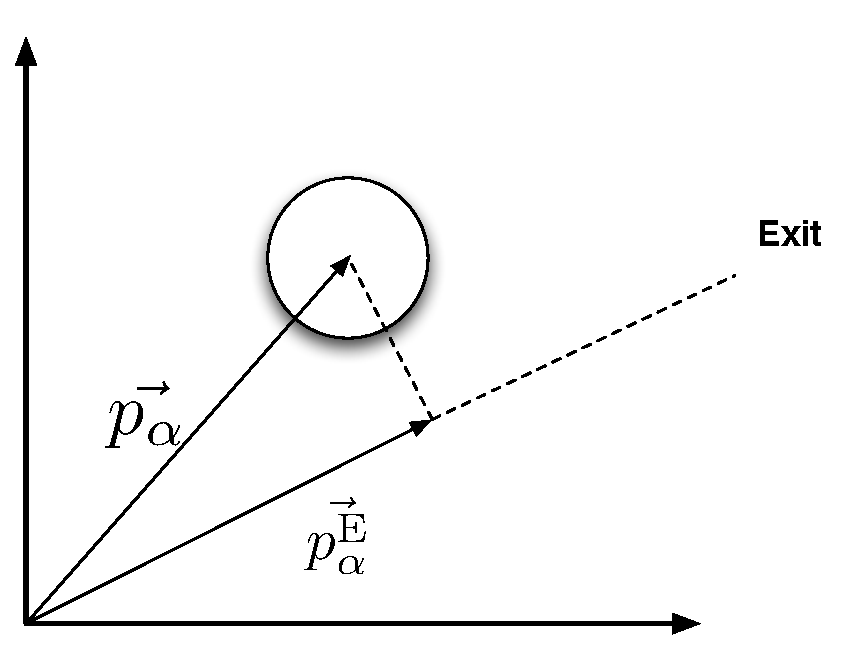
\includegraphics[width=0.5\textwidth]{Figures/NotationOfPedestrian2.pdf}} 
    \caption[Our interpretation of the average velocity]{Our interpretation of 
    the average velocity. The vector pointing from the pedestrian's initial 
    position, $p^i_\alpha$, is projected onto the vector pointing from 
    $p^i_\alpha$ to the pedestrian's target. The length of this projection is 
    divided by the time to yield the average speed.}
    \label{impatience}
\end{figure}

$\langle V_{\alpha}\rangle$ is undefined at $t=0$ as that would result in a 
division by zero. This means that $V^d_\alpha(0)$ is undefined. We correct 
this by defining $V^d_\alpha(0)=V^{Id}_\alpha$. This means that $V^d_\alpha(t)$ 
is defined as follows:

\begin{equation}\label{eqn:cond-define}
    V_{\alpha}^{d} (t) = \left\{ 
    \begin{array}{l l}
        V_\alpha^{Id} & \text{if $t=0$}\\
        \left( 1 - \eta_{\alpha}(t) \right) 
        V^{Id}_{\alpha} +
        \eta_{\alpha}(t) V_{\alpha}^{\text{max}}
        & \text{if $t > 0$}\\
    \end{array} \right.
\end{equation}

Analysing equations~\eqref{eqn:desired-speed} and \eqref{eqn:impatience}, it 
is clear that as the average speed approaches $V^{Id}_\alpha$ so does the 
desired speed, since $\eta_\alpha(t)\rightarrow0$ for $\langle V_\alpha(t) 
\rangle \rightarrow V^{Id}_\alpha$ which makes $V^d_\alpha(t)$ be dominated by 
$V^{Id}_\alpha$.  


If $\eta_\alpha(t)$ is considered as a function of the average velocity 
instead of the time, it is monotonously decreasing. This means that 
$V^d_\alpha(t)$ considered as a function of the average velocity is 
monotonously decreasing if $V^{\text{max}}_\alpha > V^{Id}_\alpha$, 
monotonously increasing if $V^{\text{max}}_\alpha < V^{Id}_\alpha$, and 
constant if $V^{\text{max}}_\alpha = V^{Id}_\alpha$. This function also has 
the property that $V^d_\alpha(t)=V^{Id}_\alpha$ when $\langle V_\alpha(t) 
\rangle = V^{Id}_\alpha$.

Since $V^{\text{max}}_\alpha$ is set to be larger than $V^{Id}_\alpha$, this 
means that as the average speed goes up, the desired speed goes down.  When 
the desired speed is lower than the actual speed, this will result in a 
negative desired force due to~\eqref{eqn:desired-force}, and vice versa. The 
end result is that the desired force will act as a stabilising force, that 
accelerates the pedestrian when it's moving slower than its desired speed, and 
decelerate it when it's moving faster, but allowing for movement of up to the 
maximum desired speed to ``make up'' for lost time if the pedestrian has been 
slowed down by the other forces acting on it.

The components of the desired force are summarised in 
table~\ref{tbl:desired-force}.

\begin{table}[h]
    \centering
    \begin{tabular}{l l}
        \toprule
        \multicolumn{2}{c}{\textsf{Parameters of the desired force}}\\
        $\overrightarrow{V_{\alpha}}(t)$ & Velocity of pedestrian $\alpha$ 
        at time $t$\\
        $V_{\alpha}^{d}(t)$ & Desired speed of pedestrian $\alpha$ at time 
        $t$\\
        $V_{\alpha}^{Id}$ & Initial desired speed of pedestrian $\alpha$ \\
        $\langle V_{\alpha}(t) \rangle$ & Average speed of pedestrian 
        $\alpha$ \\
        $\tau$& Relaxation time \\
        \bottomrule
    \end{tabular}
    \caption{Summary of parameters of the desired force}
    \label{tbl:desired-force}
\end{table}

\subsection{Interaction force between pedestrians}
\label{seq:interaction-pedestrians}
The \emph{interaction force} between pedestrians is a force between each pair 
of pedestrians $\alpha$ and $\beta$. This force is calculated for $\alpha$ as 
a sum of the interaction forces for all other pedestrians. The interaction 
force is repulsive in nature, and prevents the pedestrians from overlapping or 
walking through each other.

The variant of this force that we present is slightly different from the one 
in \cite{self-org}.  The force from the article contained too parts with 
different constants but otherwise identical; however, no explanation was given 
for how to obtain one set of constants. We have written the authors of the 
article, and they suggested we use the values from a newer article, 
\cite{ABconstant}. The force presented in this article corresponds to 
collapsing the two parts given in the original article into one, and adjusting 
the constants accordingly.

The function for the interaction force between pedestrians depends on the 
position and velocity of both pedestrians, and is given by:

\begin{equation}
    \overrightarrow{f_{\alpha \beta }}(t) = 
    w\left(\theta_{\alpha \beta}\right)
    \overrightarrow{g}\left(d_{\alpha \beta}(t)\right)
    \label{eq:pedestrianinteraction}
\end{equation}

Here $\theta_{\alpha \beta}$ is the angle between the movement direction of 
$\alpha$ and the vector pointing from $\alpha$ to $\beta$ and $d_{\alpha 
\beta}$ is the distance between the centres of the pedestrians. 

$ w(\theta_{\alpha \beta})$ is given as: 

\begin{equation}
    w\left(\theta_{\alpha \beta}\right)=
    \left(
        \lambda + \left(
            1 - \lambda
        \right)
		\frac{1+\cos{\theta}}{2}
    \right) 
    \label{angleAB}
\end{equation}

Where $\lambda$ is a parameter of the model between zero and one. This means 
that $w$ is a weight between zero and one that modifies the force given by 
$\overrightarrow{g}\left(d_{\alpha \beta}(t)\right)$ by an angular component.  
When $\lambda=1$, so is $w$, and no angular modification is made. When 
$\lambda<1$, the force is modified by a weight determined by the angle, giving 
higher weights to angles closer to $0$ and lower weights to angles close to 
$\pi$. This corresponds to the pedestrian paying more attention to (and thus 
interacting more strongly with) other pedestrians in front of it, than behind 
it. The $\lambda$ parameter determines how pronounced this anisotropic 
property of the model is.

% TODO: we should make a drawing of this.

The interaction force, $\overrightarrow{g}\left(d_{\alpha \beta} (t)\right)$, is 
given by:  

\begin{equation}
    \overrightarrow{g} 
    \left(
        d_{\alpha \beta}
    \right)
    =
    A e^{ \left(
        \frac{ R_\alpha + R_\beta - d_{\alpha \beta}}
             {B}
    \right)}
    \overrightarrow{u_{\beta \alpha}}
    \label{re}	
\end{equation}

Here $\overrightarrow{u_{\beta \alpha}}$ is the unit vector pointing from 
$\beta$ to $\alpha$ and $A$ and $B$ are model parameters. In the original 
article it is specified that they may vary between pedestrians. However, in 
practice they have a single value, so we treat them as such. The notation for 
the interaction force is summarised in 
figure~\ref{subfig:notation-interaction}.

\begin{figure}[h]
    \centering
    \subfloat[Notation for interaction]{
        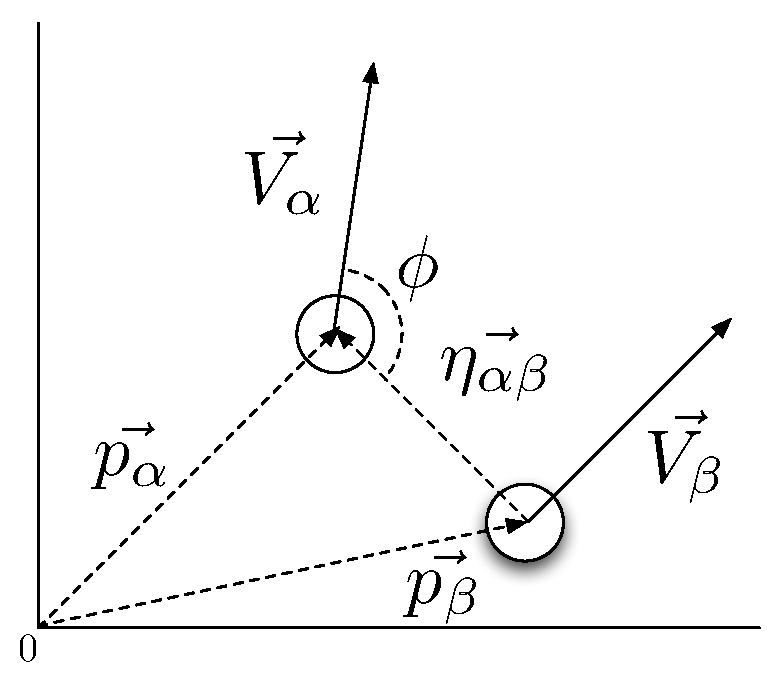
\includegraphics[width=0.45\textwidth]{Figures/NotationOfInteraction.pdf}
        \label{subfig:notation-interaction}
    } 
    \subfloat[Relation between distance and force]{
        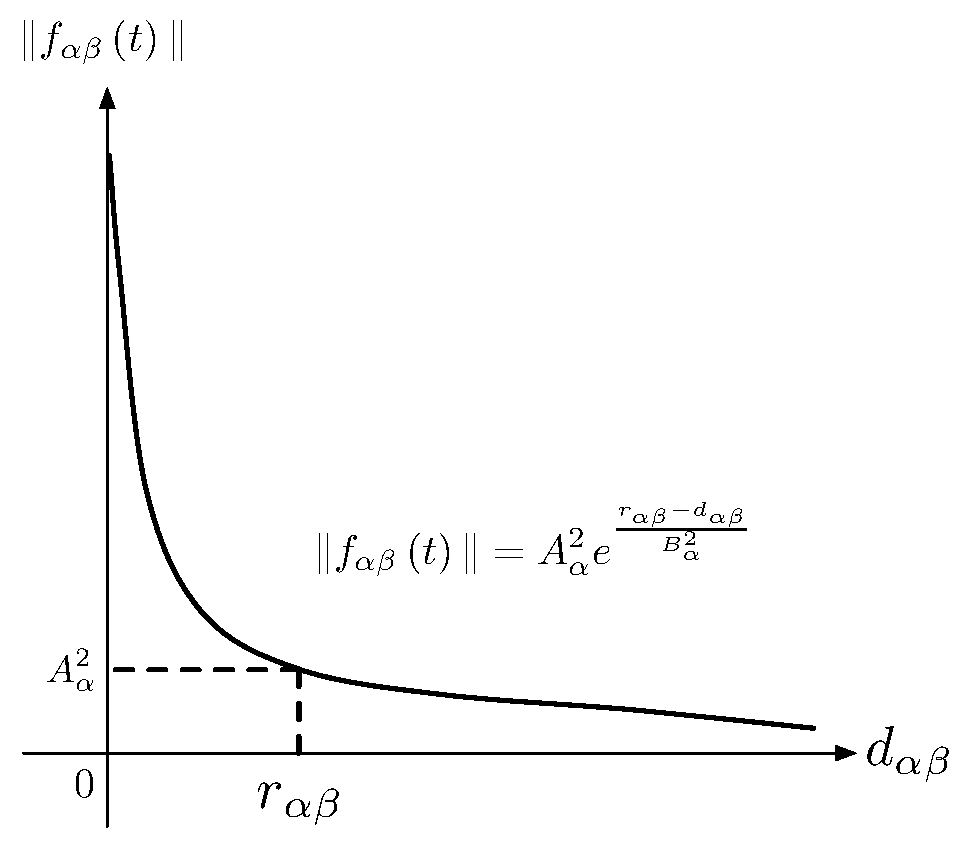
\includegraphics[width=0.45\textwidth]{Figures/physicalinteraction.pdf}
        \label{subfig:interaction-relation}
    } 
    \caption[Interaction between two pedestrians]{Interaction between two 
    pedestrians. \subref{subfig:notation-interaction} Notation of the 
    interaction between pedestrians. $d_{\alpha \beta}$ is the distance 
    between pedestrians, $\overrightarrow{u_{\beta \alpha}}$ is the unit 
    vector pointing from $\beta$ to $\alpha$, $\theta$ is the angle between 
    $\alpha$'s direction of movement and the vector pointing from $\alpha$ to 
    $\beta$. \subref{subfig:interaction-relation} The repulsive force away 
    from $\beta$ increases exponentially the closer $\alpha$ gets to $\beta$.}
    \label{fig:pedestrian-interaction}
\end{figure}

The relation between the repulsive force from $\beta$ to $\alpha$ is seen in 
figure~\ref{subfig:interaction-relation}. The force increases exponentially 
the closer $\alpha$ gets to $\beta$. This means that the force will hardly be 
noticeable for pedestrians that are far away from each other, but is strong 
enough when they are close to each other to prevent them from colliding, 
without adding any physical interaction forces. The threshold for when the 
force becomes large enough to have an impact on the movement of $\alpha$ (the 
range of the force) depends on the parameter $B$. The strength of the force 
depends on the parameter $A$.

\begin{table}
    \centering
    \begin{tabular}{l l}
        \toprule
        \multicolumn{2}{c}{\textsf{Parameters of the interaction force}}\\
        $\theta_{\alpha \beta}$ & Angle between $\alpha$'s direction of 
        movement and the vector from $\alpha$ to $\beta$\\
        $d_{\alpha \beta}$& Distance between pedestrians $\alpha$ and $\beta$ \\
        $\overrightarrow{u_{\beta \alpha}}$& Unit vector pointing from $\beta$ to $\alpha$ \\
        $\lambda$& Parameter controlling the anisotropic property of the 
        interaction\\
        $A$& Parameter controlling the interaction strength \\
        $B$& Parameter controlling the range of the repulsive interaction  \\
        \bottomrule
    \end{tabular}
    \caption{Summary of parameters of the interaction force}
    \label{tbl:interaction-forces}
\end{table}

\subsection{Repulsion from the walls}
\label{seq:repulsion-walls}
The \emph{repulsive force} from the walls is the force that prevents 
pedestrians form walking into, or even through, walls in the simulation. As 
with the interaction force between pedestrians, the repulsive force from the 
walls functions without taking into account the physical forces between walls 
and pedestrians.

The repulsion from the wall $\gamma$ is given by:

\begin{equation}\label{wallpotential}
    \overrightarrow{f_{\alpha \gamma}}(t) =
    - \nabla_{\overrightarrow{p_{\alpha}}} h
    \left( d_{\alpha \gamma}(t) \right)
\end{equation}

Here $h$ is a repulsive potential and $d_{\alpha \gamma}(t)$ is the distance 
from the pedestrian to the nearest point on the wall at time $t$. 
$\nabla_{\overrightarrow{p_\alpha}}$ is the gradient of the repulsive 
potential with respect to the pedestrian's position. The notation for the wall 
interaction is summarised in figure~\ref{fig:wall-notation}.

It is not clear from the article how finding the nearest point on the wall is 
accomplished. In most cases this can be done by projecting the position of the 
pedestrian onto the line segment that defines a wall. Some complications 
arise when walls are at odd angles to pedestrians; this is discussed further 
in section~\ref{sec:repulsion-points}. In the following, we assume that the 
nearest point on the wall, $\overrightarrow{p_{\gamma \alpha}}$, is known.

\begin{figure}[ht]
    \centering
    {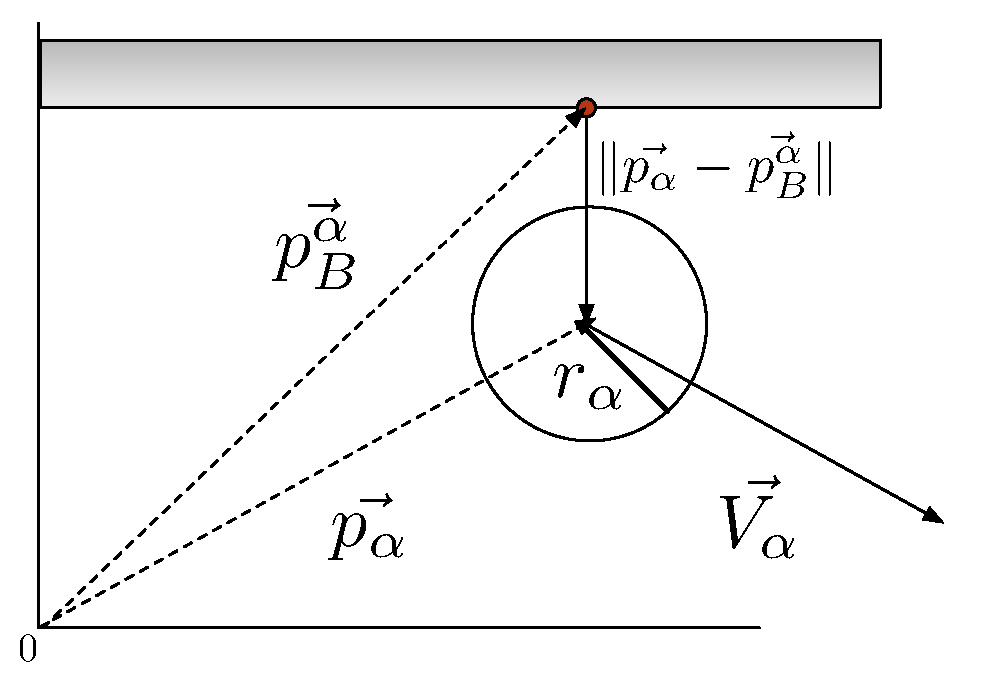
\includegraphics[width=0.5\textwidth]{Figures/NotationOfWall.pdf}} 
    \caption[Notation for the interaction between pedestrians and 
    walls]{Notation for the interaction between pedestrians and walls.  
    $\overrightarrow{p_\gamma}$ is the point on the wall $\gamma$ nearest to 
    pedestrian $\alpha$ and  $d_{\alpha \gamma}(t)$ is the distance between 
    the pedestrian and the wall.}
    \label{fig:wall-notation}
\end{figure}

The definition of $h\left( d_{\alpha \gamma}(t) \right)$ is not given in 
\cite{self-org}. However, as with the interaction force between pedestrians, 
it is given in \cite{ABconstant} by: 

\begin{equation}
    h \left( d_{\alpha \gamma}(t) \right) =
    U e^{\frac{- d_{\alpha \gamma}(t) }{ R_{\alpha} }}
\end{equation}

where $U$ is a constant given as a model parameter.

Since $p_{\gamma \alpha}$ and $p_\alpha$ are known, the gradient can be 
calculated only for the magnitude of the force, adding the direction later. 
Given this interpretation, the wall interaction force becomes:


\begin{equation}
    f_{\alpha \gamma}(t) =
    -\frac{\partial}{\partial d_{\alpha \gamma}(t)}U e^{\frac{- d_{\alpha 
    \gamma}(t) }{ R_{\alpha} }} \overrightarrow{u_{\gamma \alpha}}
\end{equation}

where $\overrightarrow{u_{\gamma \alpha}}$ is the unit vector pointing from 
$\gamma$ to $\alpha$.

Differentiating this gives: 

\begin{equation}
    f_{\alpha \gamma}(t) =
    \frac{U}{R_\alpha} 
    e^{\frac{- d_{\alpha \gamma}(t) }{ R_{\alpha} }}
    \overrightarrow{u_{\gamma \alpha}}
    \label{eqn:wall-repulsion}
\end{equation}

Since the distance between the pedestrian and the wall cannot be negative, the 
exponential term of the repulsion will always be between zero and one, rising 
towards one as the distance decreases. This means that $0 < |f_{\alpha 
\gamma}(t)| < U/R_\alpha$, increasing exponentially towards $U/R_\alpha$ as 
the distance between the pedestrian and the wall decreases. Similar to the 
interaction force between pedestrians, this means the repulsion from the walls 
is negligeble when the distance is large, but strong enough to prevent 
pedestrians from walking into or through walls even when no physical forces 
are present. The model parameter, $U$, determines exactly how strong this 
repulsive force is.

The parameters for the wall repulsion is summarised in 
table~\ref{tbl:wall-repulsion}.

\begin{table}[h]
    \centering
    \begin{tabular}{l l}
        \toprule
        \multicolumn{2}{c}{\textsf{Parameters for wall repulsion}}\\
        $\overrightarrow{p_{\gamma \alpha}}$ & Point on the wall $\gamma$ closest to 
        the pedestrian.\\
        $d_{\alpha \gamma}(t)$ & Distance from the wall $\gamma$ to pedestrian 
        $\alpha$. \\
        $U$ & Constant determining the magnitude of the repulsive force from 
        walls. \\
        \bottomrule
    \end{tabular}
    \caption{Summary of parameters for wall repulsion.}
    \label{tbl:wall-repulsion}
\end{table}

\subsection{Summary}
As we have seen, the model consists of three main parts: the desired force, 
the interaction force between agents and the repulsive force from walls. The 
desired force represents the pedestrians desire to move at a certain speed, 
given as a model parameter. The force accelerates the pedestrian to this 
speed, even allowing the pedestrian to exceed this speed to catch up to lost 
time in the event of a slowdown. The interaction force prevents pedestrians 
from walking into each other. It is a repulsive force between pedestrians that 
decreases exponentially with the distance to each other. Model parameters 
determines the magnitude and range of the force. Finally, the repulsive force 
from the walls prevents pedestrians from bumping into and walking through 
walls. This force, like the interaction force, decreases exponentially with 
distance, and its magnitude is determined by a model parameter.

A complete summary of the model's notation and parameters is given in 
table~\ref{tbl:model-summary}.

Our review of the model has revealed various areas that we need to address in 
order to create practical numerical simulations. We have already filled out 
some gaps by adding details from articles other than the original, but the 
model as we have presented it in this article is still quite abstract. In the 
following section, we outline the parts missing to turn the model into a 
simulation, and how we've solved these problems.


\begin{table}[h]
    \centering
    \begin{tabular}{l l}
        \toprule
        \multicolumn{2}{c}{\textsf{Main forces}}\\
        $\overrightarrow{f_{\alpha}^{d}}$ & Desired force\\
        $\overrightarrow{f_{\alpha \beta}}$ & Interaction force from pedestrian 
        $\beta$\\
        $\overrightarrow{f_{\alpha \gamma}}$ & Repulsive force from wall 
        $\gamma$\\

        \midrule
        \multicolumn{2}{c}{\textsf{Base notation}}\\
        $\overrightarrow{p_{\alpha}}$ & Position vector of pedestrian 
        $\alpha$\\
        $\overrightarrow{V_{\alpha}}$ & Velocity of pedestrian $\alpha$ \\ 
        \addlinespace[0.3em]
        $R_\alpha$ & Radius of pedestrian $\alpha$\\

        \midrule
        \multicolumn{2}{c}{\textsf{Parameters of the desired force}}\\
        $\overrightarrow{V_{\alpha}}(t)$ & Velocity of pedestrian $\alpha$ 
        at time $t$\\
        $V_{\alpha}^{d}(t)$ & Desired speed of pedestrian $\alpha$ at time 
        $t$\\
        $V_{\alpha}^{Id}$ & Initial desired speed of pedestrian $\alpha$ \\
        $\langle V_{\alpha}(t) \rangle$ & Average speed of pedestrian 
        $\alpha$ \\
        $\tau$& Relaxation time \\

        \midrule
        \multicolumn{2}{c}{\textsf{Parameters of the interaction force}}\\
        $\theta_{\alpha \beta}$ & Angle between $\alpha$'s direction of 
        movement and the vector from $\alpha$ to $\beta$\\
        $d_{\alpha \beta}$& Distance between pedestrians $\alpha$ and $\beta$ \\
        $\overrightarrow{u_{\beta \alpha}}$& Unit vector pointing from $\beta$ to $\alpha$ \\
        $\lambda$& Parameter controlling the anisotropic property of the 
        interaction\\
        $A$& Parameter controlling the interaction strength \\
        $B$& Parameter controlling the range of the repulsive interaction  \\

        \midrule
        \multicolumn{2}{c}{\textsf{Parameters for wall repulsion}}\\
        $\overrightarrow{p_{\gamma \alpha}}$ & Point on the wall $\gamma$ closest to 
        the pedestrian.\\
        $d_{\alpha \gamma}(t)$ & Distance from the wall $\gamma$ to pedestrian 
        $\alpha$. \\
        $U$ & Constant determining the magnitude of the repulsive force from 
        walls. \\
        \bottomrule
    \end{tabular}
    \caption{Summary of the model.}
    \label{tbl:model-summary}
\end{table}

